\section{Structured Modeling}
%\ikehata{The titles of section 3 and section 4 are quite similar. Is
%that on purpose?}
% \begin{table*}
% 	\caption{Properties of elements in the structured indoor scene representation. }
% 	\begin{tabularx}{160mm}{|c|X|X|}
% 		\hline Element Type & Properties & Description \\
% 		\hline\hline Room ($\textbf{R}$) &  RoomId & Index of the room\\
% 		\hline  &  PixelIdList & Pixel index list\\ 
% 		\hline Wall ($\textbf{W}$)  & WallId &  Index of the wall\\ 
% 		\hline  &  pRoomId & Parent room index \\
% 		\hline  &  nWallId1 & Previous wall index \\ 
% 		\hline  &  nWallId2 & Next wall index \\ 
% 		\hline  &  PixelIdList & Pixel index list \\ 
% 		\hline  &  VoxelIdList & Voxel index list \\
% 		\hline  Wall Details ($\textbf{WD}$) & pWallId & Parent wall index \\
% 		\hline  &  VoxelIdList & Voxel index list  \\ 
% 		\hline Door ($\textbf{D}$) &  DoorId & Index of the door\\ 
% 		\hline  &  pWallId1 & Parent wall index (first)\\ 
% 		\hline  &  pWallId2 & Parent wall index (second) \\ 
% 		\hline  &  Corner1 & Door corners on the wall (first)\\ 
% 		\hline  &  Corner2 & Door corners on the wall (second) \\ 
% 		\hline Ceil, Floor ($\textbf{C}, \textbf{F}$) & CeilId, FloorId & Index of the ceil/floor \\
% 		\hline  & pRoomId & Parent room index\\ 
% 		\hline  &  Z & Height of the basis plane \\ 
% 		\hline  &  VoxelIdList & Voxel index list \\
% 		\hline  Ceil Details ($\textbf{CD}$) & pCeilId & Parent ceil index \\
% 		\hline  &  VoxelIdList & Voxel index list  \\ 
% 		\hline Object ($\textbf{O}$) & pRoomId & Parent room index\\ 
% 		\hline  &  PointIdList & Point index list \\ 
% 		\hline  
% 	\end{tabularx} 
% \end{table*}

The key innovation lies in the structured representation of scene
geometries, and its reconstruction framework. We represent a scene as a
``structure graph'' and conduct reconstruction as a
sequence of ``structure grammar'' applications. This section presents
these key concepts (See Fig.~\ref{fig:graph_grammar}).
%, where the grammar defines a set of rules to manipulate the structure
%graph (See Fig.~\ref{fig:graph_grammar}).

\begin{figure*}[tb]
% 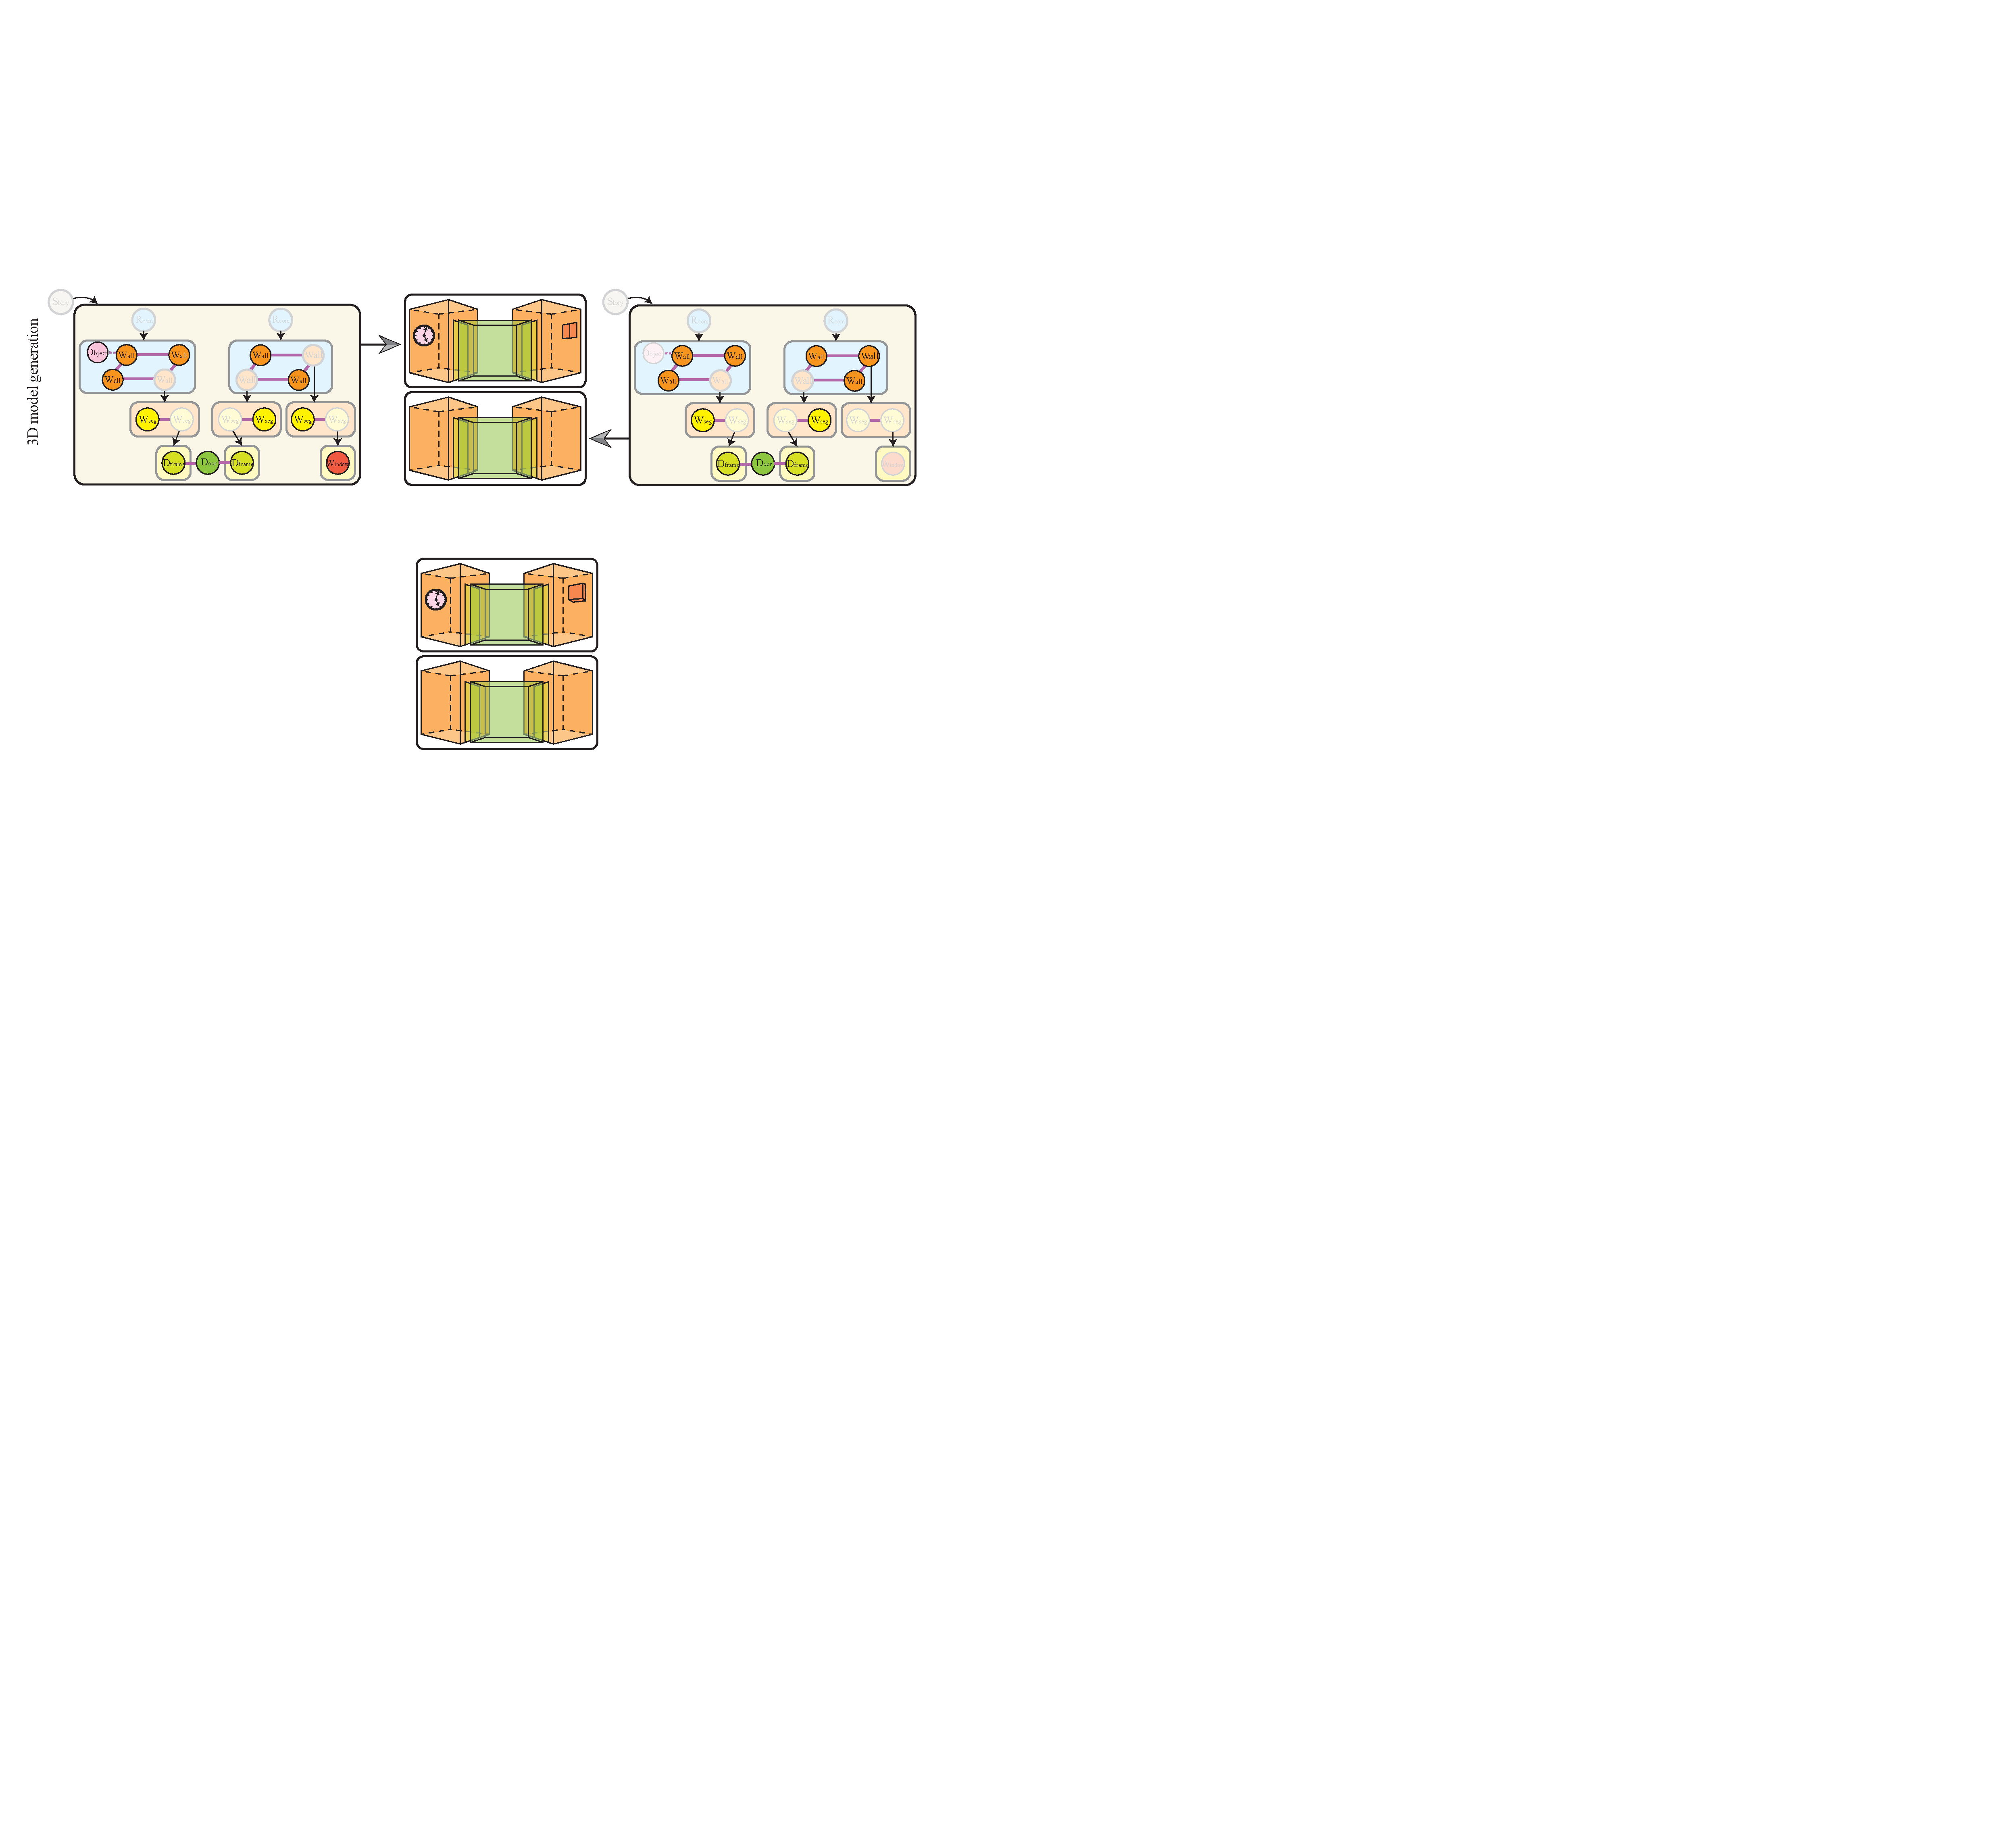
\includegraphics[width=\textwidth]{../figures/model.pdf}
\begin{center}
 \includegraphics[width=150mm]{../figures/grammar.pdf} 
 \end{center}
 \caption{Top
 left: An indoor scene is modeled as a {\em structure graph}, where
 nodes correspond to structural elements such as a room, a door, or an
 object. Each node is associated with a geometry such as a mesh or a
 depthmap, except for the scene and the room nodes. Edges contain their
 geometric relationships. A mesh model can be generated from the graph
 by outputting a mesh from every leaf node (a node without an out-going
 directed edge). Top right: One can drop an arbitrary set of nodes from
 the leaves for the mesh generation. As long as no dangling solid
 undirected edges remain, the mesh is guaranteed to be a
 manifold. Bottom: {\em Structure grammar} defines a set of possible
 transformations of this graph. Our reconstruction process is
 to sequentially apply these rules to recover the structure graph.}
 \label{fig:graph_grammar}
 \vspace{-0.325cm}
\end{figure*}

\mysubsubsection{Structure graph}
%\subsection{Structure graph}
A scene geometry is represented as a graph, where nodes correspond to
structural elements such as a room, a wall, and an object. Each node is
associated with geometry (e.g., a mesh, a depthmap, or voxels)
with the exception of ``scene'' and ``room'', which are abstract
elements. Our model works with any geometric representation, and even
allows different representations for different elements (e.g., a solid
for a room and a mesh for an object).

Nodes are connected by three types of edges.
%First, there are two types of undirected edges.
First, when structural elements have a common surface boundary (e.g.,
adjacent wall nodes), the nodes are connected by a solid undirected edge
(purple in Fig.~\ref{fig:graph_grammar}), enforcing that the geometries
match exactly along the boundary. This geometric consistency, dubbed
``boundary condition'', is the key to guarantee manifold-ness later. A
dashed undirected edge, on the other hand, represents an attachment
relationship without the boundary constraint (e.g., an object in a
room).~\footnote{We attach objects to room nodes. Give more precise
contact relationships, the framework allows one to attach to other nodes
easily (\eg, floor).}  Lastly, a directed edge encodes the
level-of-detail relationship: Structural elements at the children nodes
constitute a detailed version of the element at their parent. For
example in Fig.~\ref{fig:graph_grammar}, a ``Wall'' node contains a
simple quad surface. The child node ``Wall w/ hole''
contains a hole in the middle of the quad to represent the doorway.
% parent is a ``Wall'' node representing a simple quad surface.
Note that the boundary condition of a parent must be also satisfied by
the children nodes to guarantee the manifold-ness.

%In the above example, ``Wall'' has a boundary condition with the floor
%and the adjacent wall nodes, which must be also satisfied by the child
%node ``Wall w/ hole''.
%
% This boundary
% condition must be also satisfied by the child node ``Wall w/ hole'' so
% that the underlying scene representation exhibits a manifold regardless
% of the level of detail.
% %For example, a pair of adjacent walls are connected by this edge.


\mysubsubsection{Structure grammar}
%\subsection{Structure grammar}
Structure grammar defines a set of transformation rules that are allowed
on a structure graph, where each rule application triggers a
reconstruction algorithm. A rule has two components. 1) A
``pre-condition'' must be satisfied by the current graph to be
applicable. 2) The ``transformation'' describes how the
structure graph should change.
%
Take a room reconstruction for example. The rule takes a room node
(pre-condition). The rule produces a floor node, a ceiling node (not
shown to avoid clutter), and a chain of wall nodes (transformation).
The details of the rule set are given in Sect.~\ref{section:room}.

\mysubsubsection{Structured reconstruction}
%\subsection{Structured reconstruction}
The grammar drives our structured reconstruction process,
where the grammar rules are sequentially applied to recover a structure
graph together with the geometries. For each rule application, we choose
a geometric representation and a reconstruction algorithm that are
suitable for the task. For example, the room reconstruction rule
recovers a 1D polygon shape and extrudes it to the floor and the ceiling
heights to reconstruct a room model. The 1D polygon is obtained by a
special algorithm that is designed to produce a piecewise planar compact
polygon~\cite{Cabral2014}.
%
%This algorithm based on the dynamic programming is optimized to produce
%piecewise planar compact polygon, which is ideal to reconstruct a room
%shape.
Two types of geometric constraints need to be enforced in the
reconstruction process. First, boundary conditions must be satisfied: 1)
Existing boundary conditions (i.e., undirected solid edges) before the
rule application must be preserved; 2) New boundary conditions must be
satisfied. Second, reconstructed geometries must not intersect with the
existing geometries in the other nodes.
%The wall detail reconstruction, on the other hand, uses a 2D offset-map
%as the representation, where the combination of 2D Markov Random
%Field~\cite{label_cost_paper?} and Robust PCA~\cite{robust_pca}
%algorithms is used as the solver.
Although these constraints may appear very complex, it is fairly
straightforward to enforce them, as shown in Sect.~\ref{section:room}.

\mysubsubsection{Mesh compilation} While the structure graph is flexible
and allows different geometric representations at different nodes, it is
often desirable to produce a mesh model for applications.
%A manifold mesh enables more interesting applications as shown in
%Sect.~\ref{section:applications}.
The graph allows one to compile a manifold mesh by simply producing the
mesh geometry from each leaf node (i.e., a node without an out-going
directed edge). In the top left of Fig.~\ref{fig:graph_grammar},
non-leaf nodes are grayed-out. Here, the geometry at each node needs to
be converted to a mesh if necessary, which is easy for standard
geometric representations (e.g., a depthmap by simple meshing, a
volumetric scalar field by the Marching-Cube method~\cite{MarchingCube},
or a point cloud by Poisson Surface
Reconstruction~\cite{shan2014occluding}). Furthermore,
complexity and details of the mesh model can be easily controlled by dropping an arbitrary set of nodes from the
leaves. Since the boundary constraint at any node is satisfied by the
children, we can inductively prove that the compiled mesh model would
also be a manifold, as long as no dangling solid undirected edges
remain. Please see the supplementary material for the full proof.


\mysubsubsection{Assumptions} We assume that a scene has a single story
and that the room structure (i.e., floor, ceiling, and walls) is aligned
with the Manhattan directions. However, this restriction is due to our
particular choice of a structure grammar and reconstruction
algorithms. One can certainly change the grammar and algorithms to
extend the capabilities (e.g., multi-story and non-Manhattan buildings).
%
%\begin{figure}[!t]
%\begin{center}
%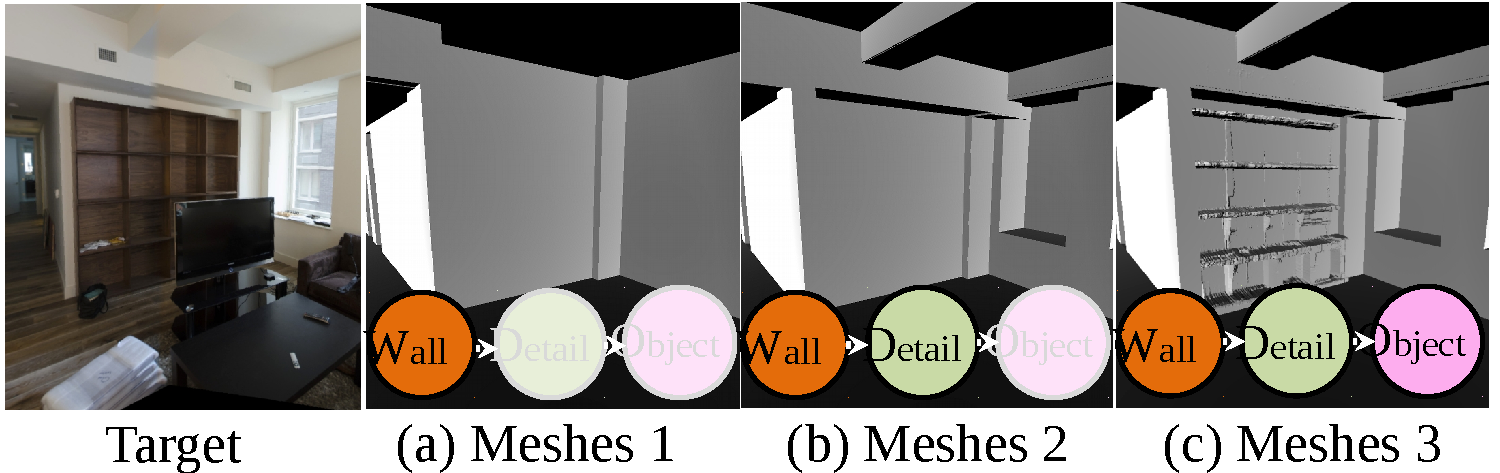
\includegraphics[width=85mm]{../figures/complexity.pdf}
%\end{center}
%\caption{We can compile the manifold meshes from a structured graph by
% changing the deepest nodes to be compiled. Here we show three examples
% where (a) wall nodes, (b) wall and their children detail nodes, and (c)
% wall, detail, and object nodes are compiled. \yasu{object is point
% cloud and technicall not a mesh. we need to be careful in using the
% word manifold and mesh, here. }}
%\label{fig:complexity1}
% \vspace{-0.25cm}
%\end{figure}

% For example in Fig.~\ref{fig:graph_grammar}, one might drop all the
% objects in one room, all the wall details from another. A proof of
% manifold-ness is given in the supplementary material.


% 3D models encoded in our graph representation can be generated at
% various levels-of-details as a manifold. The most detailed 3D model can
% be obtained by simply collecting every leaf node and outputting the
% associated geometry (the bottom left of Fig. 2). It is also easy to
% generate a 3D model without the full details. First, one can simply drop
% a part of the graph that is connected by the ``dashed'' horizontal edges
% (e.g., remove a clock from a wall). Second, one can contract any
% sub-tree, as long as the contraction does not leave any dangling
% horizontal edges.

% One can also go beyond standard model generation and create a 2D
% floorplan image from this representation, where symbolic visualization
% is preferred. One can draw 2D lines in a top down view from wall
% geometries, and place symbolic icons for other elements such as windows,
% doors, and objects.

